\section{Related Work}
\label{sec:related}

Efforts to automate seizure scoring divide by the signal they read. We position our
study against three such lines, each treated at length in the
supplementary survey (App.~\ref{sec:survey}). That survey is organized by modality,
covering EEG-only (App.~\ref{sec:eeg}), video-only (App.~\ref{sec:video}) and fused
video--EEG (App.~\ref{sec:fusion}) work, and by subject (human \vs\ animal). Its gap
analysis (App.~\ref{sec:taxonomy}, Table~\ref{tab:gap}) locates our contribution.

% Declared here so the float prints on the Related Work page, beside the
% multimodal video--EEG paragraph that first cites it.
\begin{figure}[t]
\centering
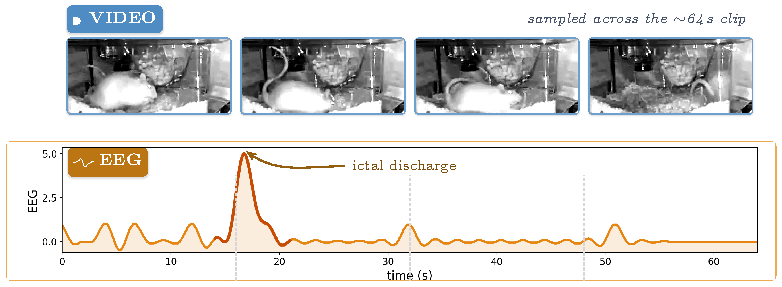
\includegraphics[width=\linewidth]{fig/fig_paired.pdf}
\caption{Synchronized video--EEG for one Stage-3 seizure clip (subject R7). \emph{Top:}
four frames sampled across the clip (contrast-enhanced), aligned to the shared time
axis. \emph{Bottom:} the simultaneous single-channel EEG ($\sim$64\,s), the shaded
window marking the ictal discharge. Video carries the convulsive motion, EEG the
electrographic discharge; this pairing is what our study rests on. De-identified.}
\label{fig:paired}
\end{figure}

\noindent\textbf{EEG-only detection} is the incumbent and sets the accuracy bar.
Rodent systems have moved from hand-crafted spectral features with classical
classifiers~\cite{bergstrom2013} to end-to-end deep networks: spectrogram CNNs
over thousands of hours~\cite{martin2023} and recurrent GRU/LSTM models that
outperform Random Forest and XGBoost on chemically diverse
cohorts~\cite{ganguly2025}. All operate on EEG alone and discard the synchronized
video recorded alongside it. We adopt this family as a deliberately strong seven-model EEG reference for our
cross-modal comparison: a GRU, an LSTM, EEGNet, an EEG Conformer, a TCN, and the
two classical baselines.

\noindent\textbf{Video-only seizure detection} reframes the task as action
recognition, inheriting mature video-understanding backbones (two-stream, 3D and
(2+1)D convolutions, and video transformers~\cite{simonyan2014twostream,
carreira2017i3d,tran2018r2plus1d,feichtenhofer2019slowfast,
bertasius2021timesformer,tong2022videomae}; reviewed in App.~\ref{sec:backbones})
and animal pose
estimators~\cite{mathis2018deeplabcut,pereira2022sleap}. Clinical video systems
target \emph{binary} recognition~\cite{ahmedt2018,karacsony2020seizure,vsvig2024};
in rodents, camera-only detectors have been built for PTZ-induced
mice~\cite{sabnis2024}, chronic-epilepsy screening~\cite{epidetect2024}, home-cage
behavioral monitoring~\cite{jankovic2019homecage} and further mouse~\cite{khan2024mice}
and zebrafish~\cite{whytefagundes2025zebrafish} preparations, and
Perlo~\etal\ recently released \emph{RodEpil}~\cite{rodepil2025}, the first public
video-only rodent benchmark (13{,}053 clips, 19 rats) with a TimeSformer baseline
at 97\% F1 under subject-wise cross-validation. We validate our backbone on
RodEpil directly and extend beyond binary detection to severity grading.

\noindent\textbf{Multimodal video--EEG fusion} is the clinical gold standard.
Figure~\ref{fig:paired} shows the two streams on one clip from our cohort: the
convulsive motion in the frames and the ictal discharge in the trace mark the same
event, and an expert confirms a seizure only by reading them together.
Computationally the pairing is rare, however: only a handful of human studies fuse
both streams~\cite{aghaei_video_eeg,martini2021,cao2024,vepinet2024}, and in animals
just two isolated attempts: late fusion of video, ECoG and piezo in
rats~\cite{mullen2024}, and cross-attention alignment of self-supervised EEG and
video in mice~\cite{eegvfusion2026}. Both address only \emph{binary} detection;
neither grades severity, the harder three- and five-class problem we study. We leave fusion to future work (Sec.~\ref{sec:open}); our aim here is to establish
how far each single modality gets on its own.
